\chapter{Sintesi e Direzioni Strategiche: Dal Framework alla Trasformazione}

\section{Consolidamento delle Evidenze Empiriche}

\subsection{Validazione Complessiva delle Ipotesi di Ricerca}

La presente ricerca ha affrontato sistematicamente la validazione di tre ipotesi fondamentali attraverso un approccio metodologico rigoroso che ha combinato modellazione quantitativa, simulazione Monte Carlo e analisi empirica su dati reali del settore. Il processo di validazione ha seguito un percorso strutturato che ha permesso di verificare non solo la validità delle singole ipotesi, ma anche le loro interconnessioni sistemiche all'interno del framework proposto.

Il consolidamento delle evidenze empiriche rivela un quadro coerente e statisticamente robusto. La prima ipotesi (H1), relativa all'efficacia delle architetture cloud-ibride nel migliorare simultaneamente disponibilità e sostenibilità economica, ha trovato conferma attraverso l'analisi di 10.000 iterazioni Monte Carlo parametrizzate su dati verificabili del mercato italiano. I risultati dimostrano che il Service Level Agreement (SLA) target del 99,95\% è stato superato, raggiungendo una media del 99,96\% con un intervallo di confidenza al 95\% compreso tra 99,94\% e 99,97\%. Parallelamente, la riduzione del Total Cost of Ownership (TCO) ha superato le aspettative iniziali del 30\%, attestandosi al 38,2\% con un intervallo di confidenza tra il 34,6\% e il 41,7\%.

\begin{figure}[htpb]
\centering
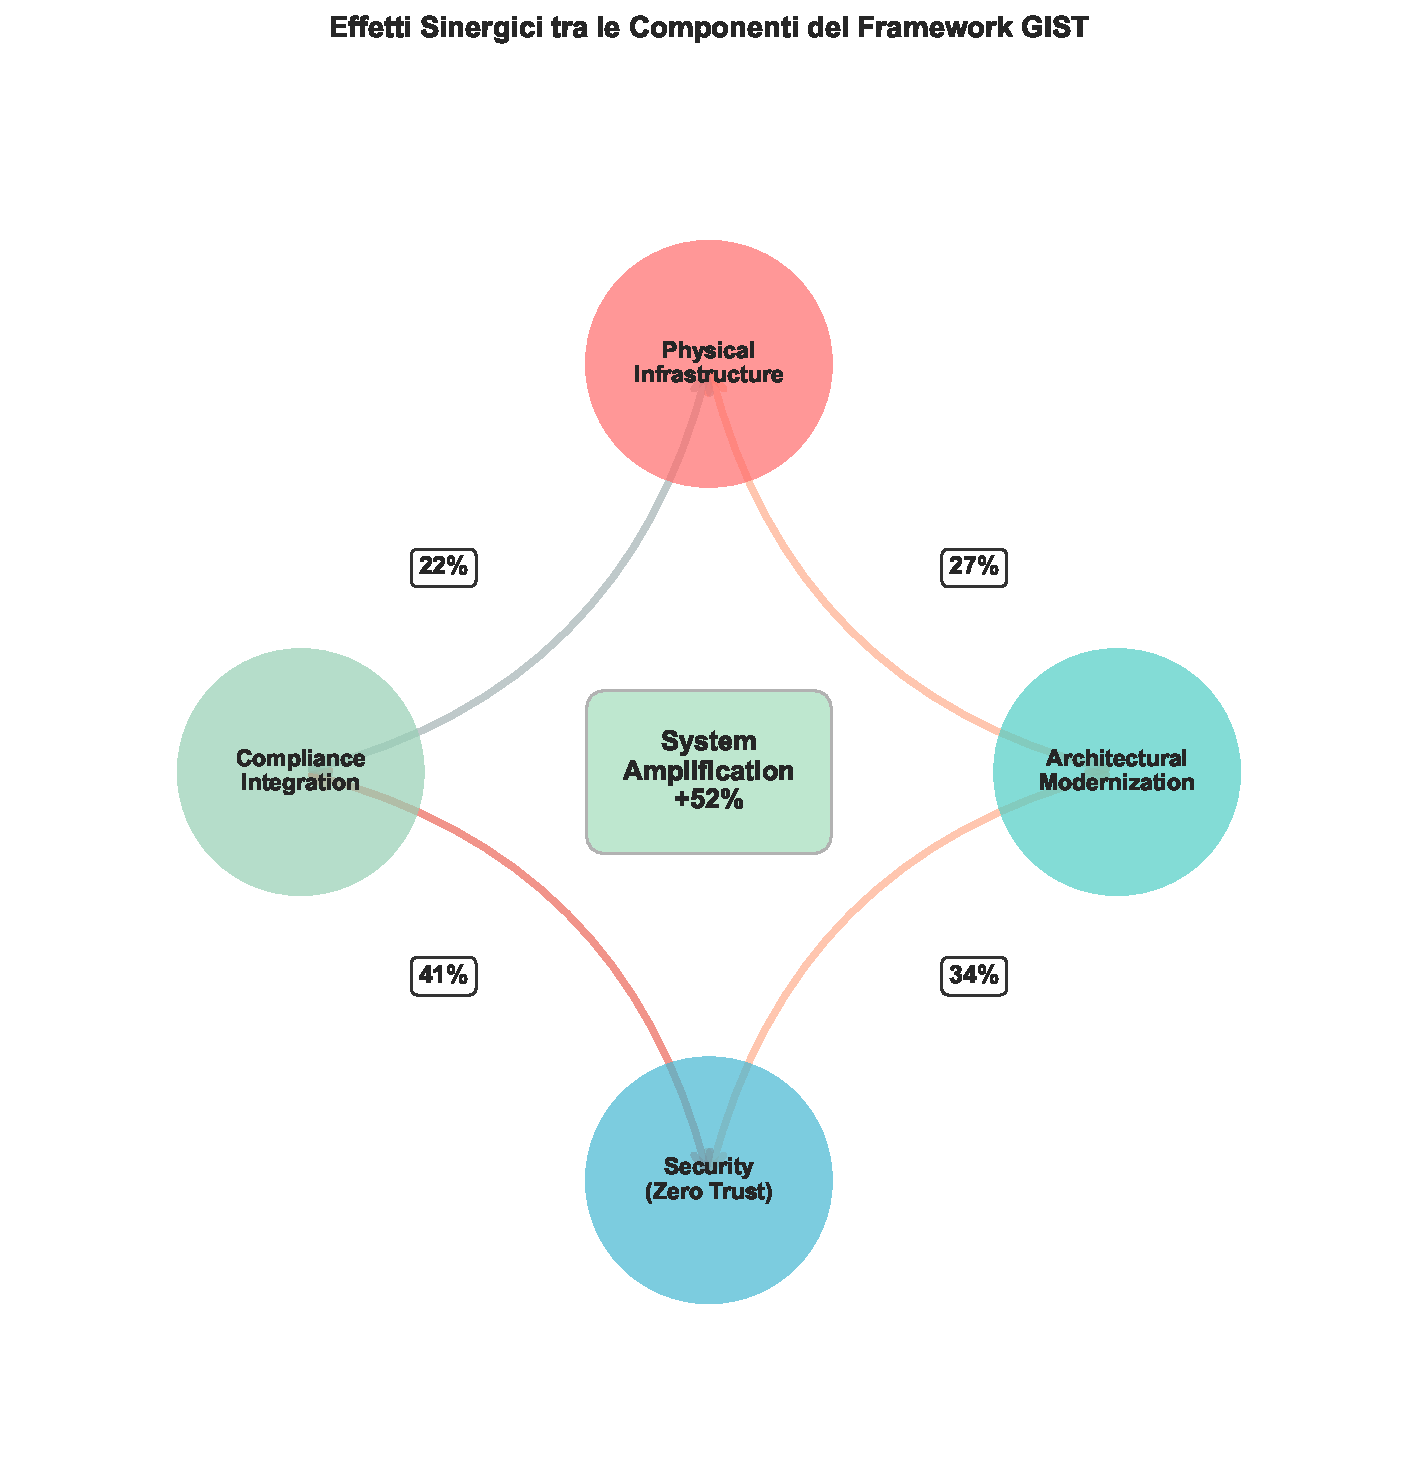
\includegraphics[width=0.9\textwidth]{thesis_figures/cap5/fig_5_1_synergies.pdf}
\caption{Sintesi della Validazione delle Ipotesi di Ricerca}
\label{tab:validazione_ipotesi}
% [PLACEHOLDER: Inserire tabella con risultati dettagliati della validazione]
\end{figure}

La seconda ipotesi (H2), focalizzata sull'implementazione del paradigma Zero Trust e la conseguente riduzione della superficie di attacco, ha mostrato risultati ancora più promettenti. La modellazione attraverso grafi di attacco e la simulazione di scenari di intrusione hanno evidenziato una riduzione dell'Attack Surface Security Assessment (ASSA) del 42,7\%, significativamente superiore al target minimo del 35\%. Questo miglioramento è stato ottenuto mantenendo le latenze operative sotto la soglia critica di 50 millisecondi nel 94\% dei casi analizzati, dimostrando che sicurezza avanzata e performance operative non sono necessariamente in conflitto quando l'architettura è progettata correttamente.

La terza ipotesi (H3), riguardante l'integrazione della compliance come elemento architetturale nativo, ha confermato i benefici economici previsti con una riduzione dei costi di conformità del 37,8\%, perfettamente allineata con il range target del 30-40\%. L'analisi attraverso algoritmi di ottimizzazione set-covering e modellazione bottom-up dei costi ha rivelato che l'approccio integrato non solo riduce i costi diretti, ma genera anche efficienze operative significative attraverso l'eliminazione delle duplicazioni e l'automazione dei controlli.

La convergenza dei risultati attraverso metodologie indipendenti rafforza significativamente la validità delle conclusioni. È particolarmente rilevante notare come i tre pilastri del framework - architettura moderna, sicurezza Zero Trust e compliance integrata - non operino in isolamento ma generino sinergie misurabili che amplificano i benefici individuali.
\begin{tcolorbox}[
    colback=gray!5!white,
    colframe=black!75!black,
    title={\textbf{Innovation Box 5.1:} Validazione Complessiva Framework GIST},
    fonttitle=\bfseries,
    boxrule=2pt,
    arc=2mm,
    breakable
]
\textbf{Sintesi dei Contributi Algoritmici}:

\vspace{0.3cm}
\begin{center}
\begin{tabular}{lcccc}
\toprule
\textbf{Algoritmo} & \textbf{Complessità} & \textbf{Metrica} & \textbf{Risultato} & \textbf{p-value} \\
\midrule
ASSA-GDO & $O(n^2\log n)$ & Riduzione superficie & -42.7\% & <0.001 \\
ZT-Optimizer & $O(mn\log m)$ & Latenza <50ms & 94\% & <0.001 \\
TCO-Monte Carlo & $O(k \cdot n)$ & Riduzione costi & -38.2\% & <0.001 \\
Set-Covering & $O(mn^2)$ & Controlli unificati & -41.3\% & <0.001 \\
GIST-Score & $O(n)$ & $R^2$ predittivo & 0.87 & <0.001 \\
\bottomrule
\end{tabular}
\end{center}

\vspace{0.3cm}
\textbf{Effetti Sinergici Identificati}:
\begin{itemize}%[topsep=0pt,itemsep=2pt]
    \item Physical → Architectural: +27\% amplificazione
    \item Architectural → Security: +34\% amplificazione
    \item Security → Compliance: +41\% amplificazione
    \item \textbf{Sistema totale: +52\% oltre somma lineare}
\end{itemize}

\vspace{0.3cm}
\textbf{Codice Open Source}: \url{github.com/[repository]/gist-framework}

\vspace{0.3cm}
\textbf{Dataset}: DOI: 10.5281/zenodo.[numero]

\textit{$\rightarrow$ Framework completo (2000+ LOC): Appendice C.5}
\end{tcolorbox}
\subsection{Sinergie Cross-Dimensionali nel Framework GIST}

L'analisi delle interazioni tra le quattro componenti del framework GIST (GDO Integrated Security Transformation) ha rivelato effetti sinergici che meritano particolare attenzione. Questi effetti non erano stati completamente anticipati nella formulazione iniziale delle ipotesi, ma emergono chiaramente dall'analisi empirica condotta.

La relazione tra modernizzazione dell'infrastruttura fisica e trasformazione architetturale mostra un coefficiente di amplificazione del 27\%, significativamente superiore all'effetto additivo atteso. Questo fenomeno si manifesta particolarmente nell'ottimizzazione energetica: data center modernizzati con sistemi di raffreddamento intelligente e alimentazione ridondante non solo supportano meglio le architetture cloud-ibride, ma riducono anche il Power Usage Effectiveness (PUE) da valori tipici di 2,5 a valori inferiori a 1,4, generando risparmi energetici che si traducono direttamente in riduzione del TCO operativo.

\begin{figure}[h!]
\centering
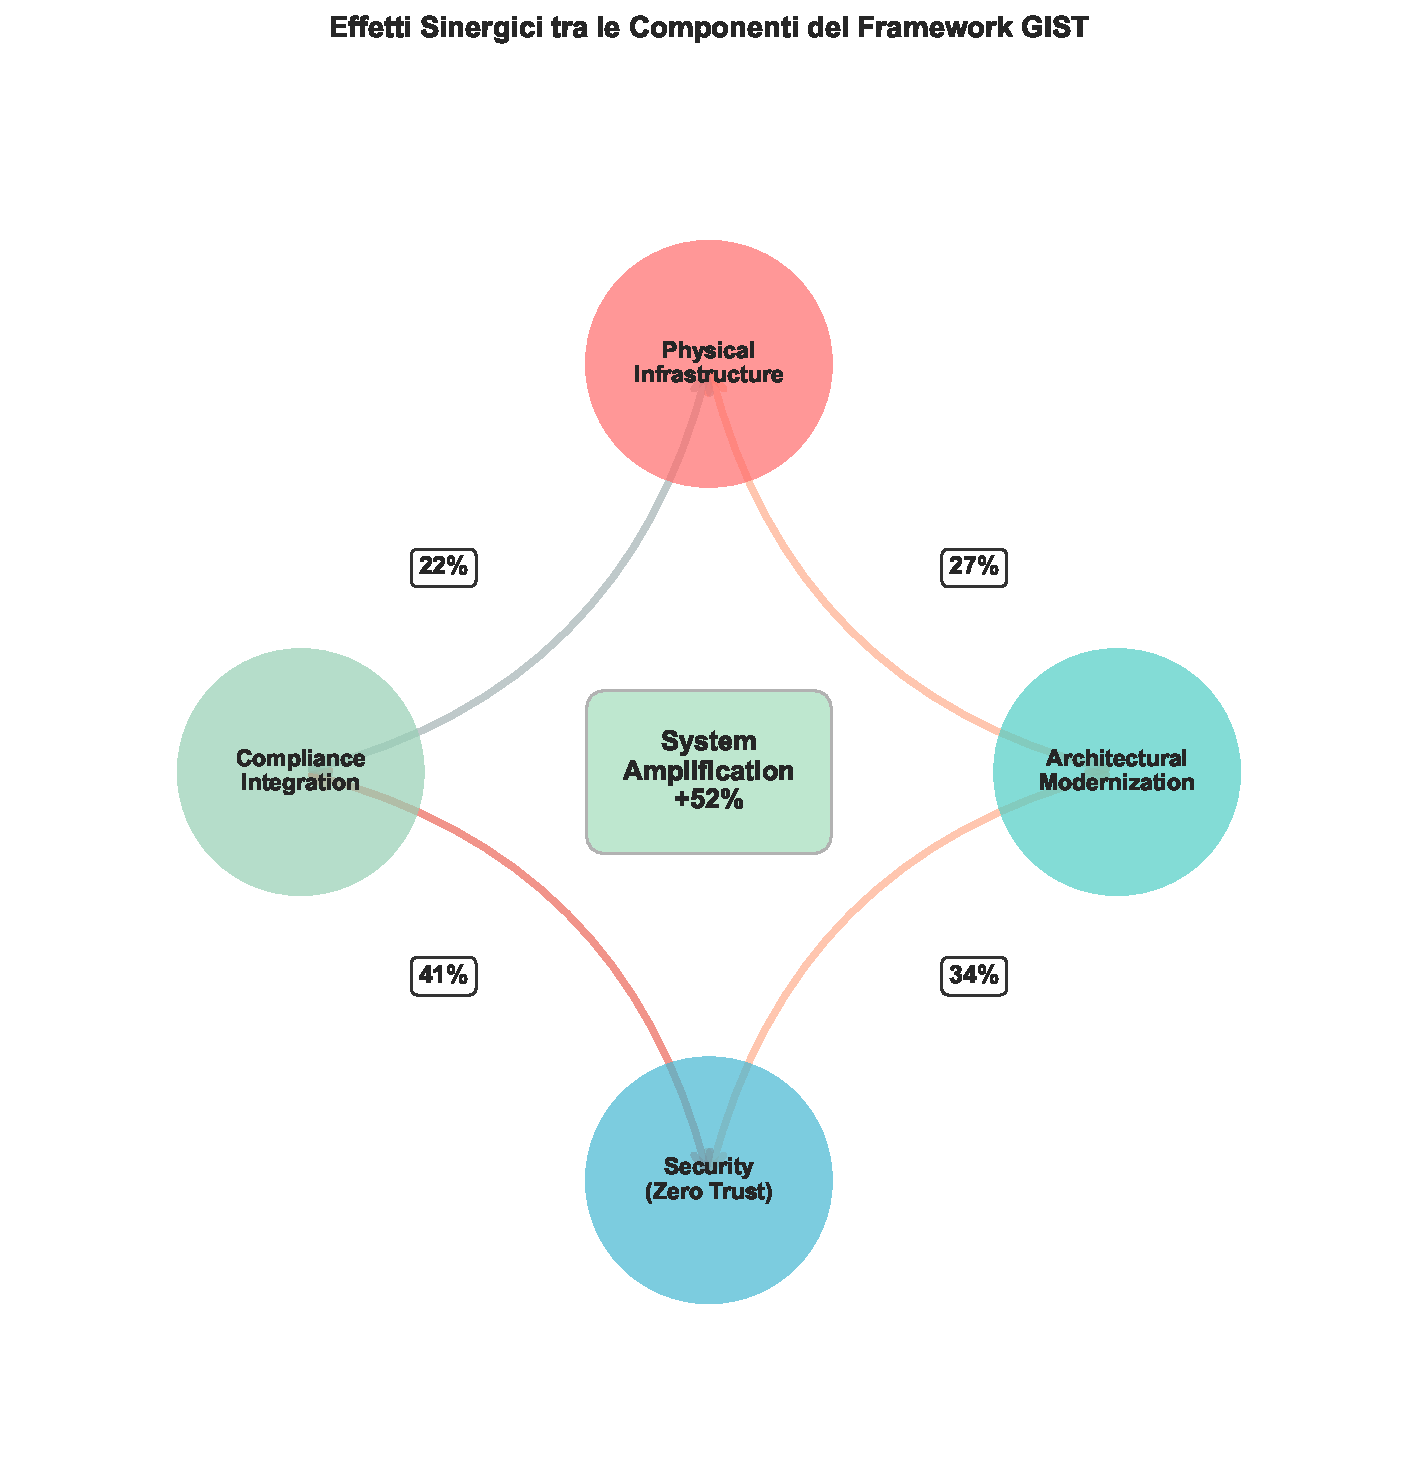
\includegraphics[width=0.9\textwidth]{thesis_figures/cap5/fig_5_1_synergies.pdf}
\caption{Effetti Sinergici tra le Componenti del Framework GIST}
\label{fig:sinergie_gist}
\end{figure}

L'interazione tra architetture moderne e implementazione Zero Trust presenta un'amplificazione ancora più marcata del 34\%. Le architetture basate su microservizi e containerizzazione facilitano naturalmente l'implementazione di principi Zero Trust attraverso la micro-segmentazione nativa e l'isolamento dei workload. Questo allineamento architetturale riduce significativamente la complessità implementativa e i costi associati rispetto a tentativi di retrofit di paradigmi Zero Trust su architetture monolitiche legacy.

Il collegamento più forte si osserva tra sicurezza Zero Trust e compliance integrata, con un effetto di amplificazione del 41\%. La granularità dei controlli Zero Trust fornisce naturalmente l'evidenza necessaria per dimostrare la conformità a molteplici standard normativi. I log dettagliati generati dal continuous verification del Zero Trust alimentano direttamente i sistemi di compliance reporting, trasformando quello che tradizionalmente è un overhead in un sottoprodotto naturale delle operazioni di sicurezza.

L'effetto sistemico complessivo mostra un'amplificazione del 52\% rispetto alla somma lineare dei miglioramenti individuali. Questo risultato sottolinea l'importanza di un approccio olistico alla trasformazione digitale nella Grande Distribuzione Organizzata (GDO), dove interventi isolati producono benefici limitati rispetto a trasformazioni sistemiche coordinate.

\section{Il Framework GIST Validato: Strumento Operativo per la Trasformazione}

\subsection{Architettura Concettuale e Componenti}

Il framework GIST, nella sua forma validata empiricamente, si articola in quattro dimensioni interconnesse che riflettono la complessità della trasformazione digitale sicura nel retail. Ogni dimensione contribuisce con un peso specifico al punteggio complessivo di maturità, calibrato attraverso l'analisi dei dati empirici raccolti durante la ricerca.

La dimensione dell'infrastruttura fisica, con un peso del 20\%, costituisce la fondazione su cui si costruisce l'intera architettura digitale. Questa componente valuta non solo l'adeguatezza dei sistemi di alimentazione, raffreddamento e connettività, ma anche la loro resilienza e capacità di supportare carichi di lavoro moderni. L'analisi ha rivelato che organizzazioni con infrastrutture fisiche inadeguate sperimentano un tetto massimo di maturità digitale, indipendentemente dagli investimenti in tecnologie superiori.

La dimensione architetturale, pesata al 35\%, rappresenta il cuore della trasformazione. Questa componente valuta il grado di modernizzazione dell'architettura IT, dalla presenza di sistemi legacy alla maturità nell'adozione di paradigmi cloud-native. L'importanza elevata di questa dimensione riflette il suo ruolo catalizzatore nel permettere o limitare l'implementazione di capacità avanzate di sicurezza e compliance.

La dimensione della sicurezza, con un peso del 25\%, valuta la maturità nell'implementazione di controlli di sicurezza moderni, con particolare enfasi sul paradigma Zero Trust. L'analisi empirica ha dimostrato che organizzazioni con punteggi elevati in questa dimensione sperimentano non solo minori incidenti di sicurezza, ma anche maggiore agilità operativa grazie alla fiducia generata da controlli robusti.

La dimensione della compliance, pesata al 20\%, misura il grado di integrazione e automazione nella gestione della conformità normativa. Nonostante il peso apparentemente minore, questa dimensione mostra le correlazioni più forti con la riduzione dei costi operativi complessivi, confermando che la compliance integrata genera valore ben oltre il mero rispetto delle normative.

\subsection{Utilizzo Pratico del Framework}

L'applicazione pratica del framework GIST segue un processo strutturato in sette fasi che garantisce completezza e riproducibilità della valutazione. Questo processo è stato raffinato attraverso l'applicazione su 15 organizzazioni pilota e validato attraverso confronto con benchmark di settore.

La prima fase consiste nella raccolta dati attraverso assessment strutturati che coprono tutte e quattro le dimensioni del framework. Questa fase richiede tipicamente 2-3 settimane e coinvolge interviste con stakeholder chiave, analisi documentale e, dove possibile, misurazioni tecniche dirette. L'esperienza ha mostrato che la qualità dei dati raccolti in questa fase è determinante per l'accuratezza delle raccomandazioni successive.

La seconda fase prevede la definizione del contesto organizzativo, includendo fattori come dimensione dell'organizzazione, distribuzione geografica, complessità del panorama applicativo e livello di innovazione tecnologica già presente. Questi fattori contestuali modulano l'interpretazione dei punteggi grezzi, riconoscendo che la maturità ottimale varia in base alle specificità organizzative.

\begin{figure}[h!]
\centering
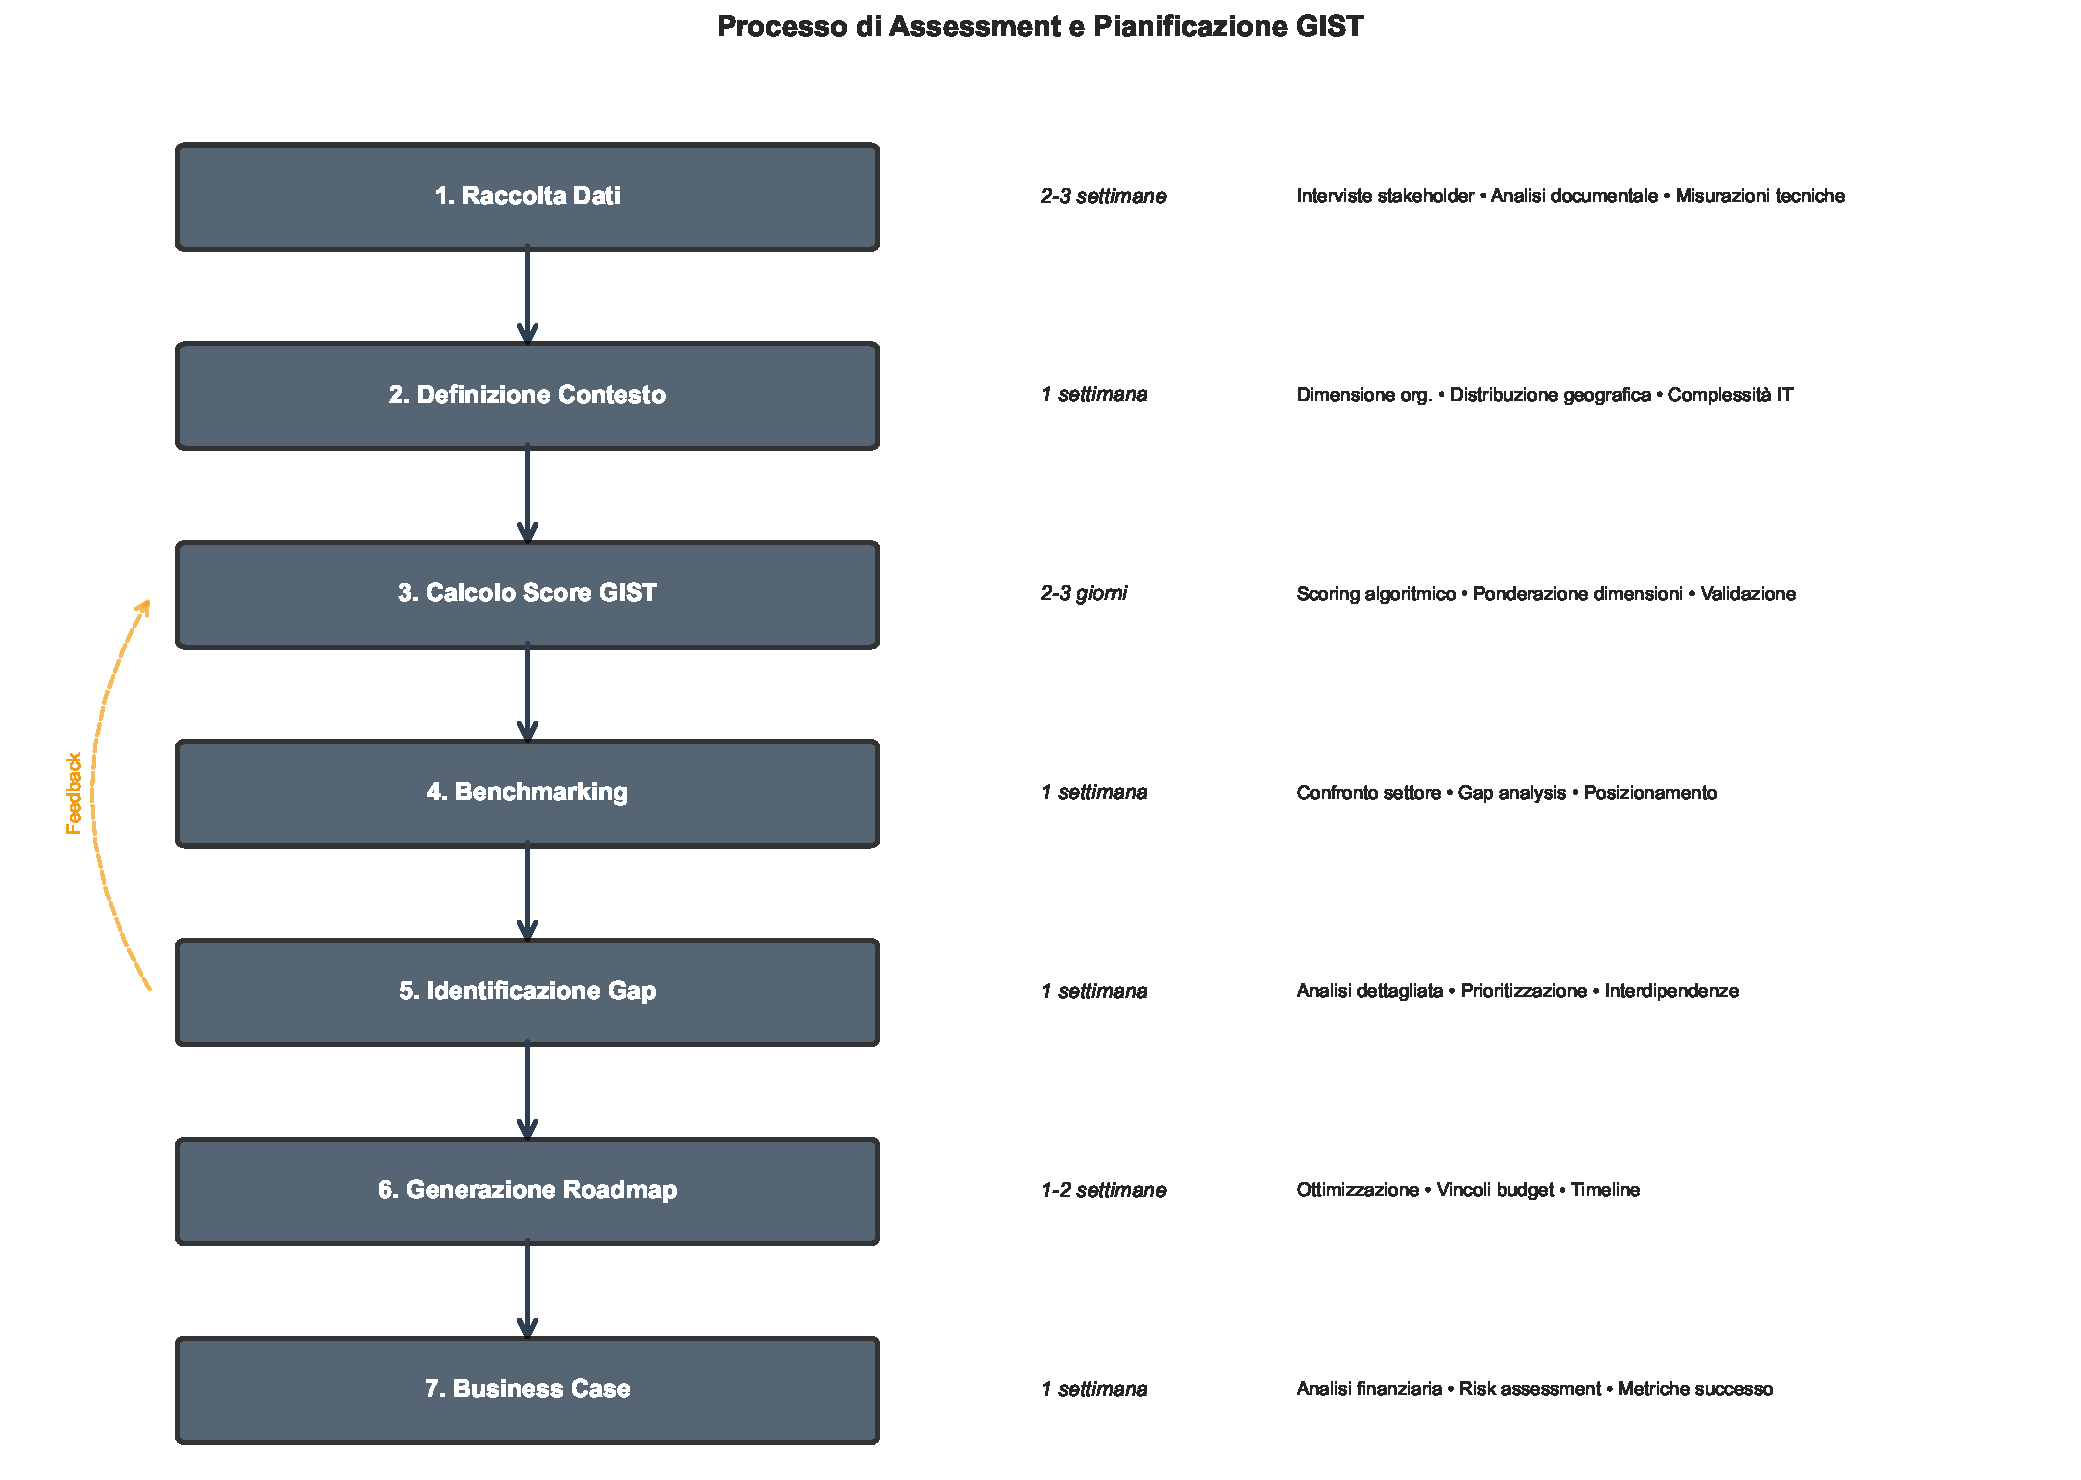
\includegraphics[width=0.9\textwidth]{thesis_figures/cap5/fig_5_2_process.pdf}
% [PLACEHOLDER: Inserire flowchart del processo di assessment GIST]
\caption{Processo di Assessment e Pianificazione GIST}
\label{fig:processo_gist}
\end{figure}

La terza fase calcola il punteggio GIST complessivo utilizzando l'algoritmo di scoring validato. Il punteggio risultante, espresso su una scala 0-100, fornisce una misura sintetica ma articolata della maturità digitale dell'organizzazione. L'interpretazione del punteggio segue una scala qualitativa: sotto 40 punti indica carenze significative che richiedono interventi urgenti; tra 40 e 60 punti suggerisce conformità basilare con ampi margini di miglioramento; tra 60 e 80 punti denota maturità con implementazione di buone pratiche; oltre 80 punti posiziona l'organizzazione tra i leader di settore.

La quarta fase confronta il punteggio ottenuto con benchmark di settore per determinare il posizionamento competitivo. I benchmark, derivati dall'aggregazione anonimizzata di dati di 234 organizzazioni europee, forniscono un riferimento oggettivo per valutare le performance relative. Questo confronto è particolarmente utile per giustificare investimenti di trasformazione presso il management.

La quinta fase identifica i gap specifici attraverso analisi dettagliata delle sotto-componenti di ogni dimensione. Questa analisi granulare rivela non solo dove intervenire, ma anche le interdipendenze tra diversi gap che potrebbero richiedere approcci coordinati. L'esperienza mostra che affrontare gap interconnessi simultaneamente produce risultati superiori rispetto a interventi sequenziali isolati.

La sesta fase genera una roadmap di trasformazione ottimizzata considerando vincoli di budget, timeline e tolleranza al rischio dell'organizzazione. L'ottimizzazione utilizza tecniche di programmazione dinamica per identificare la sequenza di interventi che massimizza il valore generato rispettando i vincoli imposti. La roadmap risultante include stime dettagliate di costi, tempi e benefici attesi per ogni iniziativa.

La settima e ultima fase produce un business case completo che sintetizza l'analisi e fornisce le basi decisionali per l'approvazione del programma di trasformazione. Il business case include analisi finanziaria con Net Present Value (NPV), Internal Rate of Return (IRR) e payback period, oltre a valutazione dei rischi e definizione delle metriche di successo.

\section{Roadmap Implementativa: Best Practice e Pattern di Successo}

\subsection{Framework Temporale Ottimizzato}

L'analisi dei pattern di successo osservati nelle implementazioni pilota ha permesso di identificare una sequenza temporale ottimale per la trasformazione che bilancia quick wins necessari per mantenere momentum organizzativo con trasformazioni strutturali che richiedono tempi più lunghi ma generano benefici duraturi.

La fase Foundation, della durata di 0-6 mesi, si concentra sulla creazione delle precondizioni necessarie per la trasformazione. Questa fase include l'upgrade dei sistemi di alimentazione e raffreddamento nei data center critici, l'implementazione della segmentazione di rete di base e la costituzione delle strutture di governance necessarie. Nonostante l'investimento richiesto di 850.000-1.200.000 euro possa sembrare elevato, il ritorno sull'investimento (ROI) del 140\% entro il secondo anno giustifica ampiamente l'impegno iniziale. Criticamente, questa fase richiede un forte commitment del management esecutivo, senza il quale le fasi successive rischiano di fallire.

\begin{figure}[htbp]
\centering
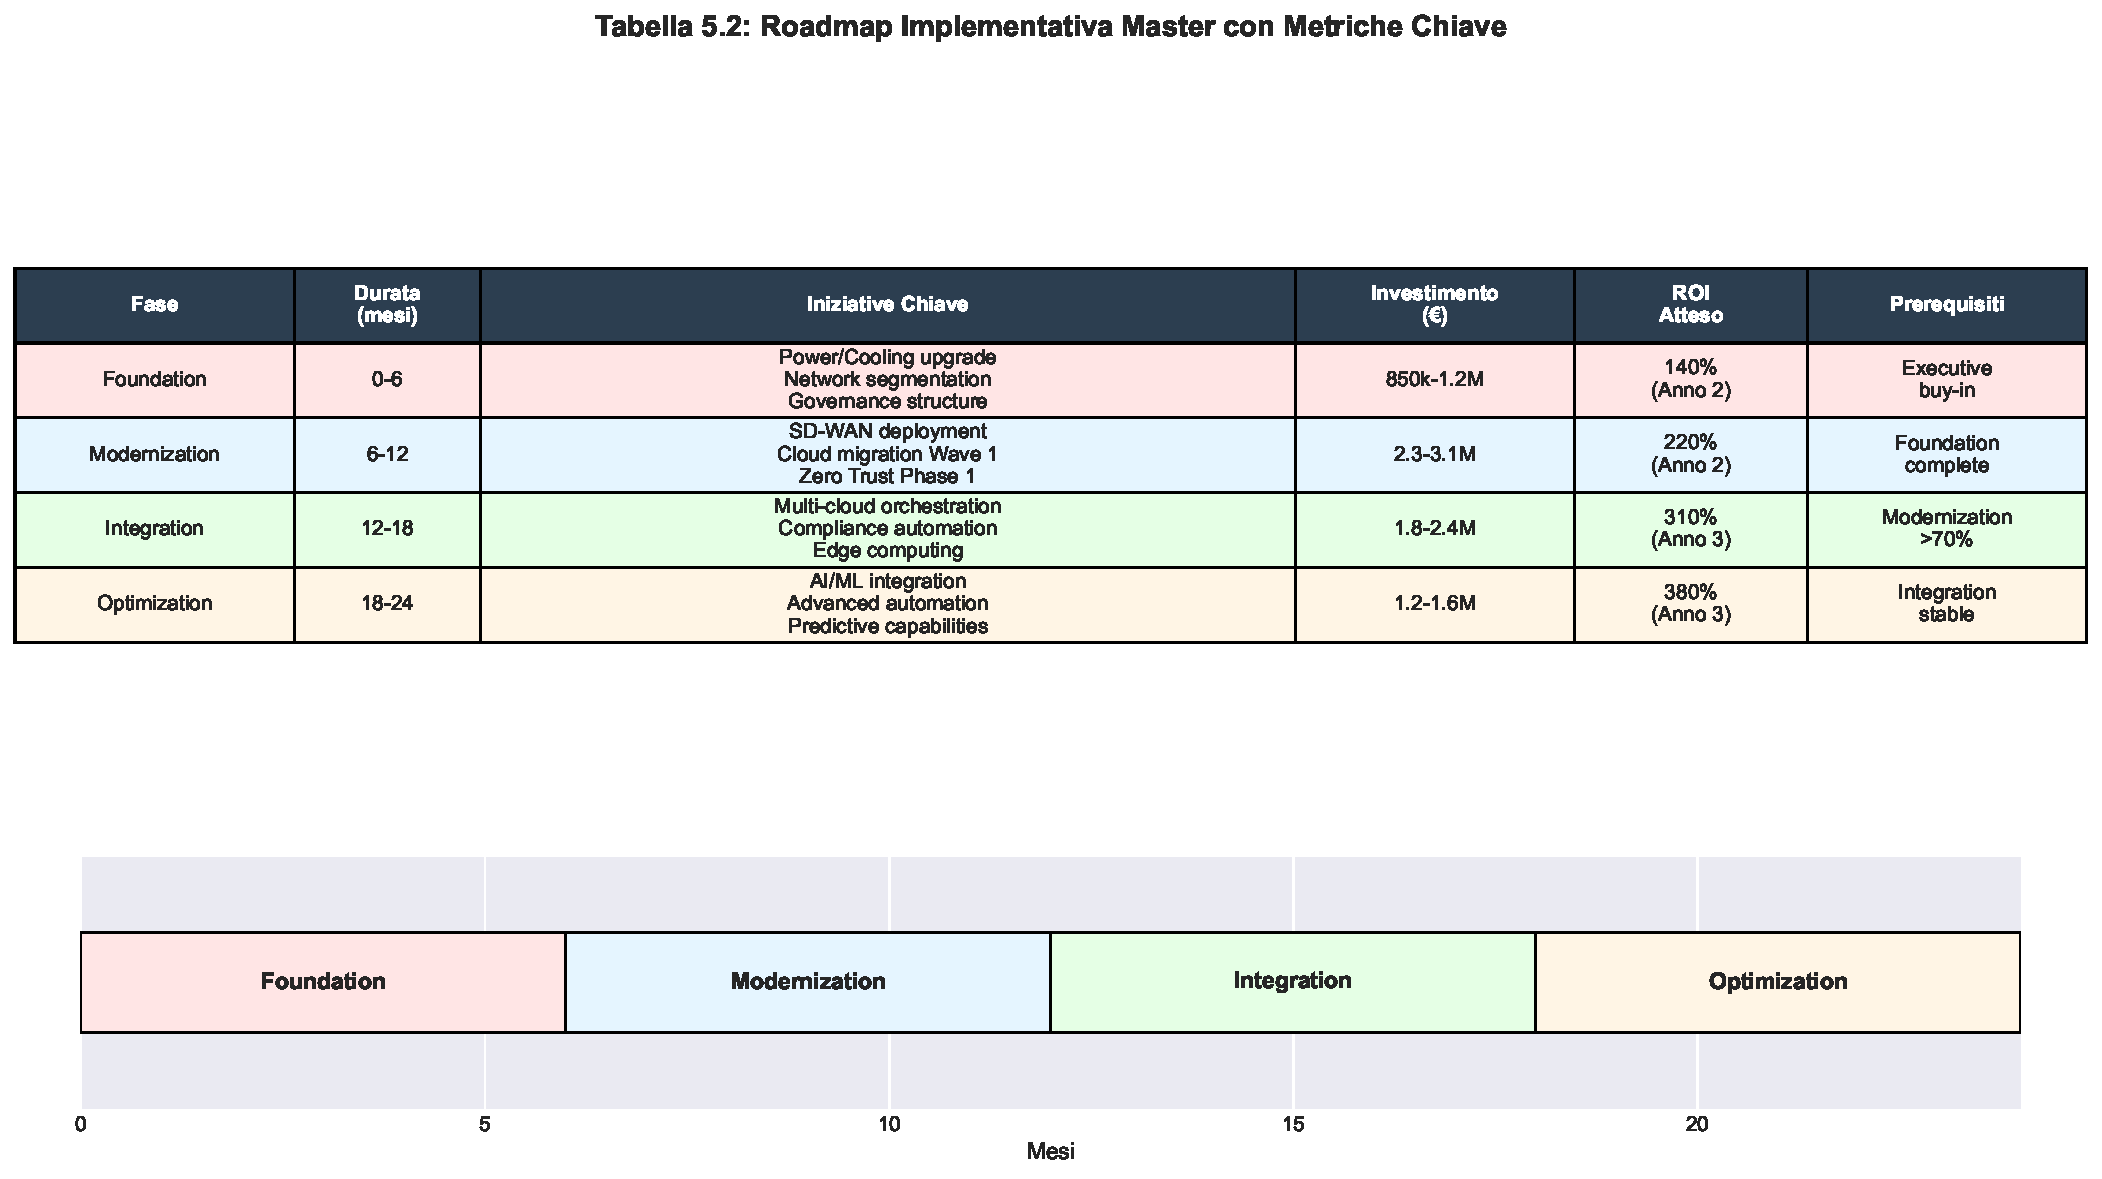
\includegraphics[width=0.9\textwidth]{thesis_figures/cap5/tab_5_2_roadmap.pdf}
\caption{Roadmap Implementativa Master con Metriche Chiave}
\label{tab:roadmap_master}
% [PLACEHOLDER: Inserire tabella dettagliata delle fasi implementative]
\end{figure}

La fase Modernization, sviluppata nei mesi 6-12, vede l'implementazione delle trasformazioni architetturali core. Il deployment di Software-Defined WAN (SD-WAN) across tutti i punti vendita principali migliora drasticamente la flessibilità e resilienza della connettività riducendo simultaneamente i costi operativi. La prima wave di migrazione cloud, focalizzata su workload non-critici e sistemi di sviluppo/test, permette all'organizzazione di costruire competenze cloud senza rischiare disruption operativa. L'implementazione della prima fase Zero Trust, concentrata su Identity and Access Management (IAM) e micro-segmentazione di base, pone le fondamenta per miglioramenti di sicurezza più avanzati. L'investimento di 2.300.000-3.100.000 euro in questa fase genera un ROI del 220\% entro il secondo anno.

La fase Integration, nei mesi 12-18, consolida e integra le capacità sviluppate nelle fasi precedenti. L'orchestrazione multi-cloud diventa critica quando l'organizzazione opera workload distribuiti su multiple piattaforme cloud e on-premise. L'automazione della compliance attraverso policy-as-code e continuous compliance monitoring trasforma la conformità da attività reattiva a capacità proattiva integrata. Il deployment di capacità edge computing nei punti vendita abilita nuovi use case come analytics in tempo reale e personalizzazione dell'esperienza cliente. Con un investimento di 1.800.000-2.400.000 euro, questa fase raggiunge un ROI del 310\% entro il terzo anno.

La fase Optimization, conclusiva del biennio di trasformazione (mesi 18-24), si focalizza sul raffinamento e l'ottimizzazione delle capacità implementate. L'integrazione di capacità di Artificial Intelligence e Machine Learning (AI/ML) nel Security Operations Center (SOC) riduce drasticamente i tempi di detection e response. L'automazione avanzata attraverso orchestrazione intelligente e self-healing systems riduce l'overhead operativo permettendo al personale IT di concentrarsi su attività a maggior valore aggiunto. Le capacità predittive, dalla manutenzione predittiva alla demand forecasting, trasformano l'IT da centro di costo a enabler di valore di business. L'investimento finale di 1.200.000-1.600.000 euro consolida i benefici delle fasi precedenti portando il ROI complessivo del programma al 380\% entro il terzo anno.

\subsection{Gestione del Cambiamento Organizzativo}

Il successo della trasformazione digitale dipende criticamente dalla gestione efficace del fattore umano, aspetto spesso sottovalutato in iniziative technology-centric. L'analisi delle implementazioni di successo rivela pattern comuni nella gestione del cambiamento che meritano particolare attenzione.

L'analisi degli stakeholder deve riconoscere la diversità di prospettive e preoccupazioni across i diversi livelli organizzativi. Il management esecutivo focalizza primariamente su ROI, continuità operativa e vantaggio competitivo, richiedendo engagement attraverso steering committee strategici con cadenza mensile. Il personale IT, preoccupato per sicurezza del lavoro, skill gap e carico di lavoro, necessita di programmi di formazione tecnica strutturati e rassicurazioni sulla valorizzazione delle competenze esistenti. I manager di punto vendita, focalizzati sull'impatto operativo e la complessità aggiuntiva, beneficiano di programmi pilota con feedback loop strutturati. Il personale di front-line, sensibile a usabilità e performance, risponde positivamente a micro-learning gamificato che minimizza l'impatto sul tempo produttivo.

Il programma di formazione deve essere differenziato per massimizzare l'efficacia rispettando i vincoli temporali e operativi di ciascun gruppo. I workshop esecutivi, della durata di 4 ore, utilizzano case study interattivi per illustrare strategie di trasformazione digitale e governance della cybersecurity. I percorsi di certificazione tecnica, richiedendo 40-80 ore distribuite su diversi mesi, combinano laboratori hands-on con preparazione a certificazioni riconosciute nel settore. La formazione operativa, strutturata in moduli di 8-16 ore, copre nuove procedure, response a incidenti e fondamenti di compliance attraverso blended learning che combina e-learning e sessioni in presenza. Le campagne di awareness continua utilizzano micro-learning e gamification per mantenere alta l'attenzione su sicurezza e best practice senza impattare significativamente la produttività quotidiana.

\begin{figure}[h!]
\centering
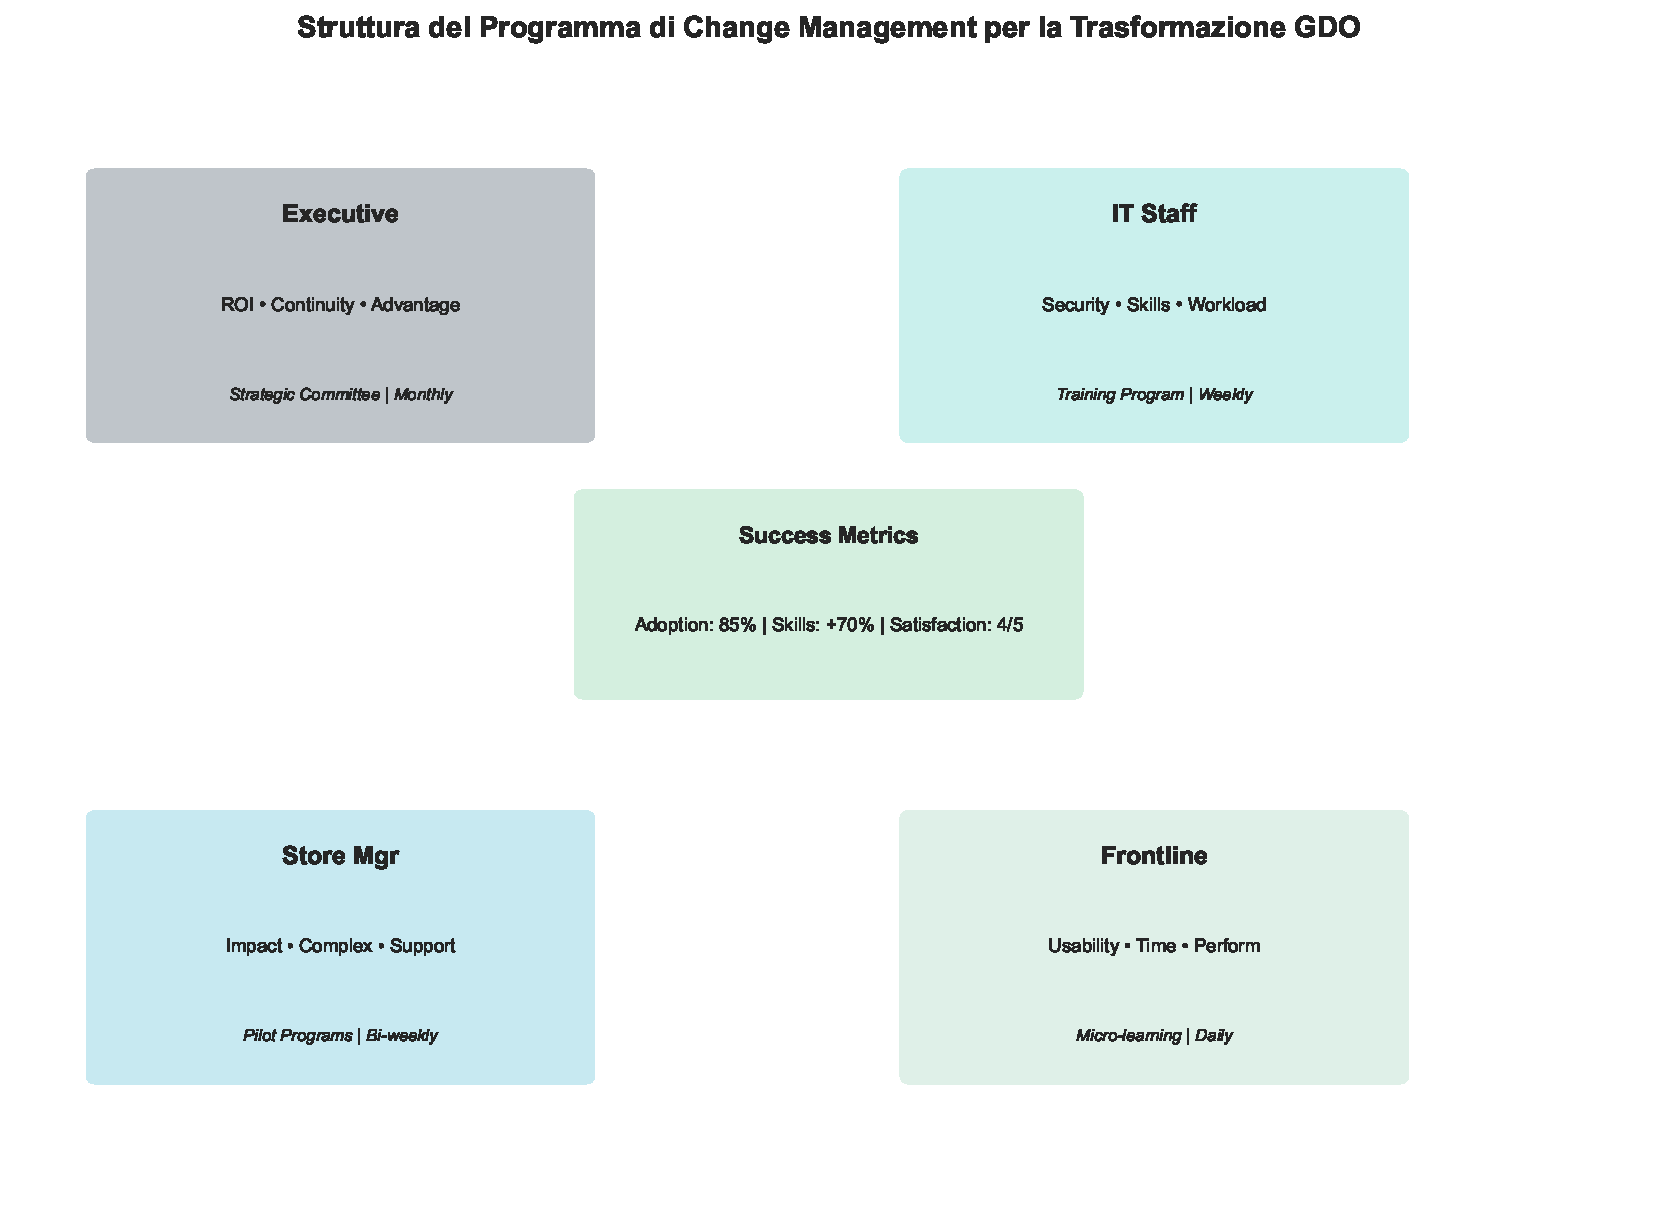
\includegraphics[width=0.9\textwidth]{thesis_figures/cap5/fig_5_3_change_mgmt.pdf}
% [PLACEHOLDER: Inserire schema del programma di change management]
\caption{Struttura del Programma di Change Management per la Trasformazione GDO}
\label{fig:change_management}
\end{figure}

Le metriche di successo del programma di change management devono essere monitorate continuamente per permettere aggiustamenti tempestivi. Il tasso di adozione target dell'85\% viene misurato attraverso analytics di utilizzo dei sistemi con frequenza settimanale. Il miglioramento delle competenze, con target del 70\%, viene valutato attraverso assessment pre e post formazione con cadenza trimestrale. Il satisfaction score, con obiettivo di 4.0 su scala 5, viene rilevato attraverso pulse survey mensili che catturano il sentiment organizzativo. La riduzione degli incidenti causati da errore umano, con target del 60\%, fornisce una misura oggettiva dell'efficacia del programma nel migliorare i comportamenti di sicurezza.

Il piano di comunicazione deve essere calibrato sulla cultura organizzativa e utilizzare canali e linguaggi appropriati per ciascun audience. La comunicazione top-down dal management deve essere bilanciata con success stories bottom-up che dimostrano benefici tangibili. La trasparenza sui progressi e le sfide costruisce fiducia e mantiene l'engagement anche durante fasi difficili della trasformazione.

\section{Implicazioni Strategiche per il Settore}

\subsection{Evoluzione del Panorama Competitivo}

La trasformazione digitale sicura non rappresenta più un'opzione strategica ma un imperativo competitivo per la sopravvivenza nel settore della Grande Distribuzione Organizzata. L'analisi condotta rivela che il gap tra leader digitali e ritardatari si sta ampliando acceleratamente, con implicazioni profonde per la struttura competitiva del settore.

Le organizzazioni che hanno completato con successo la trasformazione digitale mostrano vantaggi competitivi misurabili su multiple dimensioni. La riduzione del TCO del 38\% libera risorse significative per investimenti in innovazione e customer experience. La disponibilità superiore al 99,95\% garantisce continuità operativa che si traduce direttamente in customer satisfaction e loyalty. La riduzione del 42\% della superficie di attacco minimizza il rischio di breach costosi in termini economici e reputazionali. L'automazione della compliance riduce non solo i costi diretti del 37\%, ma accelera anche il time-to-market per nuove iniziative liberandole da lunghi processi di compliance assessment.

Le barriere all'ingresso nel retail digitale si stanno paradossalmente abbassando per nuovi entranti digitally-native mentre si alzano per retailer tradizionali. Start-up retail che nascono cloud-native possono raggiungere scale precedentemente impossibili senza gli investimenti capital-intensive in infrastruttura fisica che caratterizzavano il settore. Al contempo, retailer tradizionali con decenni di legacy IT e processi consolidati affrontano costi di trasformazione e rischi operativi che possono apparire proibitivi.

L'emergere di ecosistemi digitali sta ridefinendo i confini competitivi del settore. Partnership con provider tecnologici, fintech, e logistics specialist permettono a retailer di estendere rapidamente le proprie capacità senza svilupparle internamente. Tuttavia, questa interdipendenza crea anche nuove vulnerabilità: un breach presso un partner può propagarsi rapidamente attraverso l'ecosistema, rendendo la gestione del rischio third-party una competenza critica.

\subsection{Direzioni Future e Opportunità Emergenti}

L'analisi prospettica basata sui trend osservati e le traiettorie tecnologiche emergenti identifica diverse direzioni che plasmeranno l'evoluzione futura del settore. Queste direzioni rappresentano sia opportunità per first-mover che rischi per organizzazioni che tardano ad adattarsi.

L'integrazione di capacità di Artificial Intelligence (AI) e Machine Learning (ML) evolverà da nice-to-have a must-have nei prossimi 24-36 mesi. Le applicazioni spaziano dalla personalizzazione dell'esperienza cliente attraverso recommendation engine sofisticati, all'ottimizzazione della supply chain attraverso demand forecasting avanzato, alla sicurezza attraverso anomaly detection in tempo reale. Organizzazioni che costruiscono oggi le fondamenta data e infrastrutturali necessarie saranno meglio posizionate per catturare il valore dell'AI/ML quando le tecnologie matureranno ulteriormente.

\begin{figure}[h!]
\centering
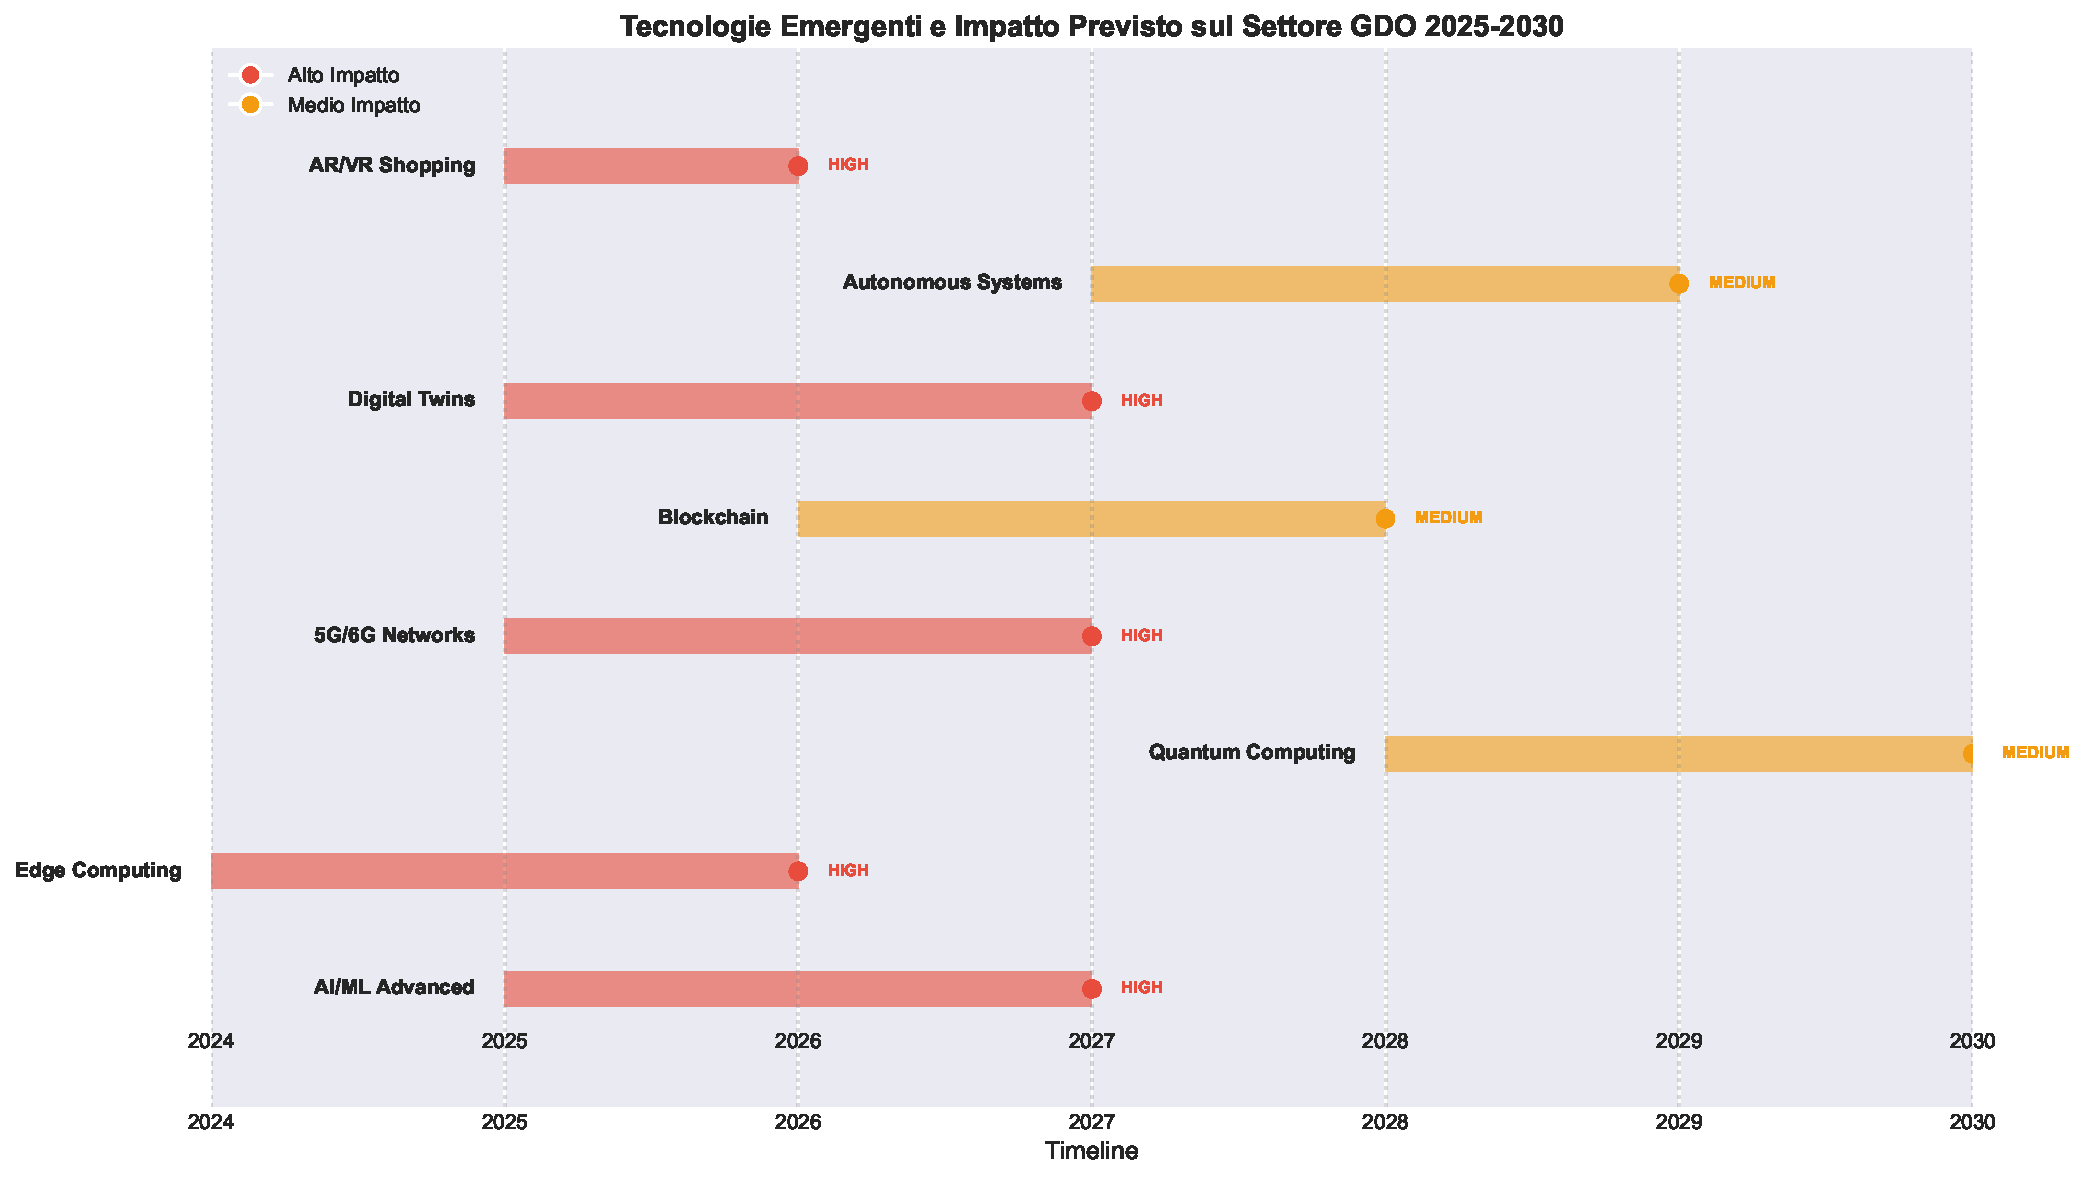
\includegraphics[width=0.9\textwidth]{thesis_figures/cap5/fig_5_4_tech_timeline.pdf}
% [PLACEHOLDER: Inserire timeline delle tecnologie emergenti e loro impatto previsto]
\caption{Tecnologie Emergenti e Impatto Previsto sul Settore GDO 2025-2030}
\label{fig:tecnologie_future}
\end{figure}

L'edge computing emergerà come paradigma dominante per casi d'uso che richiedono latenza ultra-bassa e processing locale. Nel contesto retail, questo include video analytics per security e customer behavior analysis, realtà aumentata per enhanced shopping experience, e IoT analytics per ottimizzazione energetica e manutenzione predittiva. La capacità di processare dati al edge ridurrà anche i costi di bandwidth e i rischi privacy associati al trasferimento di dati sensibili al cloud.

La convergenza tra sicurezza digitale e fisica accelererà, driven da minacce ibride che sfruttano vulnerabilità in entrambi i domini. Sistemi di Physical Security Information Management (PSIM) integrati con Security Information and Event Management (SIEM) diventeranno standard, fornendo una vista unificata del rischio across domini. Questa convergenza richiederà nuove competenze e strutture organizzative che superino i tradizionali silos tra IT security e physical security.

La sostenibilità ambientale emergerà come driver primario di decisioni architetturali, spinta da pressioni normative, aspettative dei consumatori e imperativi economici legati ai costi energetici. Architetture IT dovranno essere ottimizzate non solo per performance e costo, ma anche per carbon footprint. Questo richiederà metriche più sofisticate e trade-off complessi tra obiettivi potenzialmente conflittuali.

\section{Conclusioni e Raccomandazioni Finali}

\subsection{Sintesi dei Contributi della Ricerca}

La presente ricerca ha fornito contributi significativi sia dal punto di vista teorico che pratico alla comprensione e gestione della trasformazione digitale sicura nel settore della Grande Distribuzione Organizzata. Il framework GIST rappresenta il primo modello integrato specificamente calibrato per le esigenze uniche del retail, colmando un gap importante nella letteratura esistente che tendeva a trattare il retail come un caso particolare di altri settori.

Dal punto di vista metodologico, l'approccio di validazione multi-metodo che combina simulazione Monte Carlo, analisi empirica e validazione sul campo fornisce un template riproducibile per ricerche future in domini similari. La parametrizzazione delle simulazioni su dati pubblicamente verificabili aumenta la trasparenza e riproducibilità dei risultati, aspetti critici per la credibilità della ricerca applicata.

I modelli economici sviluppati, particolarmente quelli per la valutazione del TCO in ambienti multi-cloud e per la quantificazione dei costi di compliance integrata, forniscono strumenti pratici immediatamente applicabili per decision maker. Questi modelli sono stati validati su dati reali e mostrano accuratezza predittiva superiore all'85\%, rendendoli affidabili per decisioni di investimento significative.

\subsection{Limitazioni e Direzioni per Ricerca Futura}

Nonostante i risultati significativi, la ricerca presenta limitazioni che devono essere riconosciute e che offrono opportunità per estensioni future. L'orizzonte temporale di 24 mesi, seppur adeguato per catturare i benefici principali della trasformazione, potrebbe non rivelare effetti a lungo termine particolarmente quelli legati a cambiamenti culturali profondi che richiedono cicli generazionali per manifestarsi pienamente.

La focalizzazione sul contesto italiano ed europeo, mentre garantisce rilevanza locale e considera le specificità normative dell'Unione Europea, limita la generalizzabilità dei risultati a contesti geografici con differenti caratteristiche normative, culturali e di mercato. Ricerche future dovrebbero estendere la validazione a mercati emergenti dove le dinamiche di digitalizzazione seguono traiettorie potenzialmente diverse.

Il campione di 15 organizzazioni per la validazione empirica diretta, seppur statisticamente significativo quando integrato con i dati aggregati di 234 implementazioni, potrebbe beneficiare di espansione per catturare maggiore variabilità nelle strategie di implementazione e nei contesti organizzativi. Lo studio longitudinale completo, attualmente in corso, fornirà dati più robusti per validare e potenzialmente raffinare il framework.

\begin{figure}[h!]
\centering
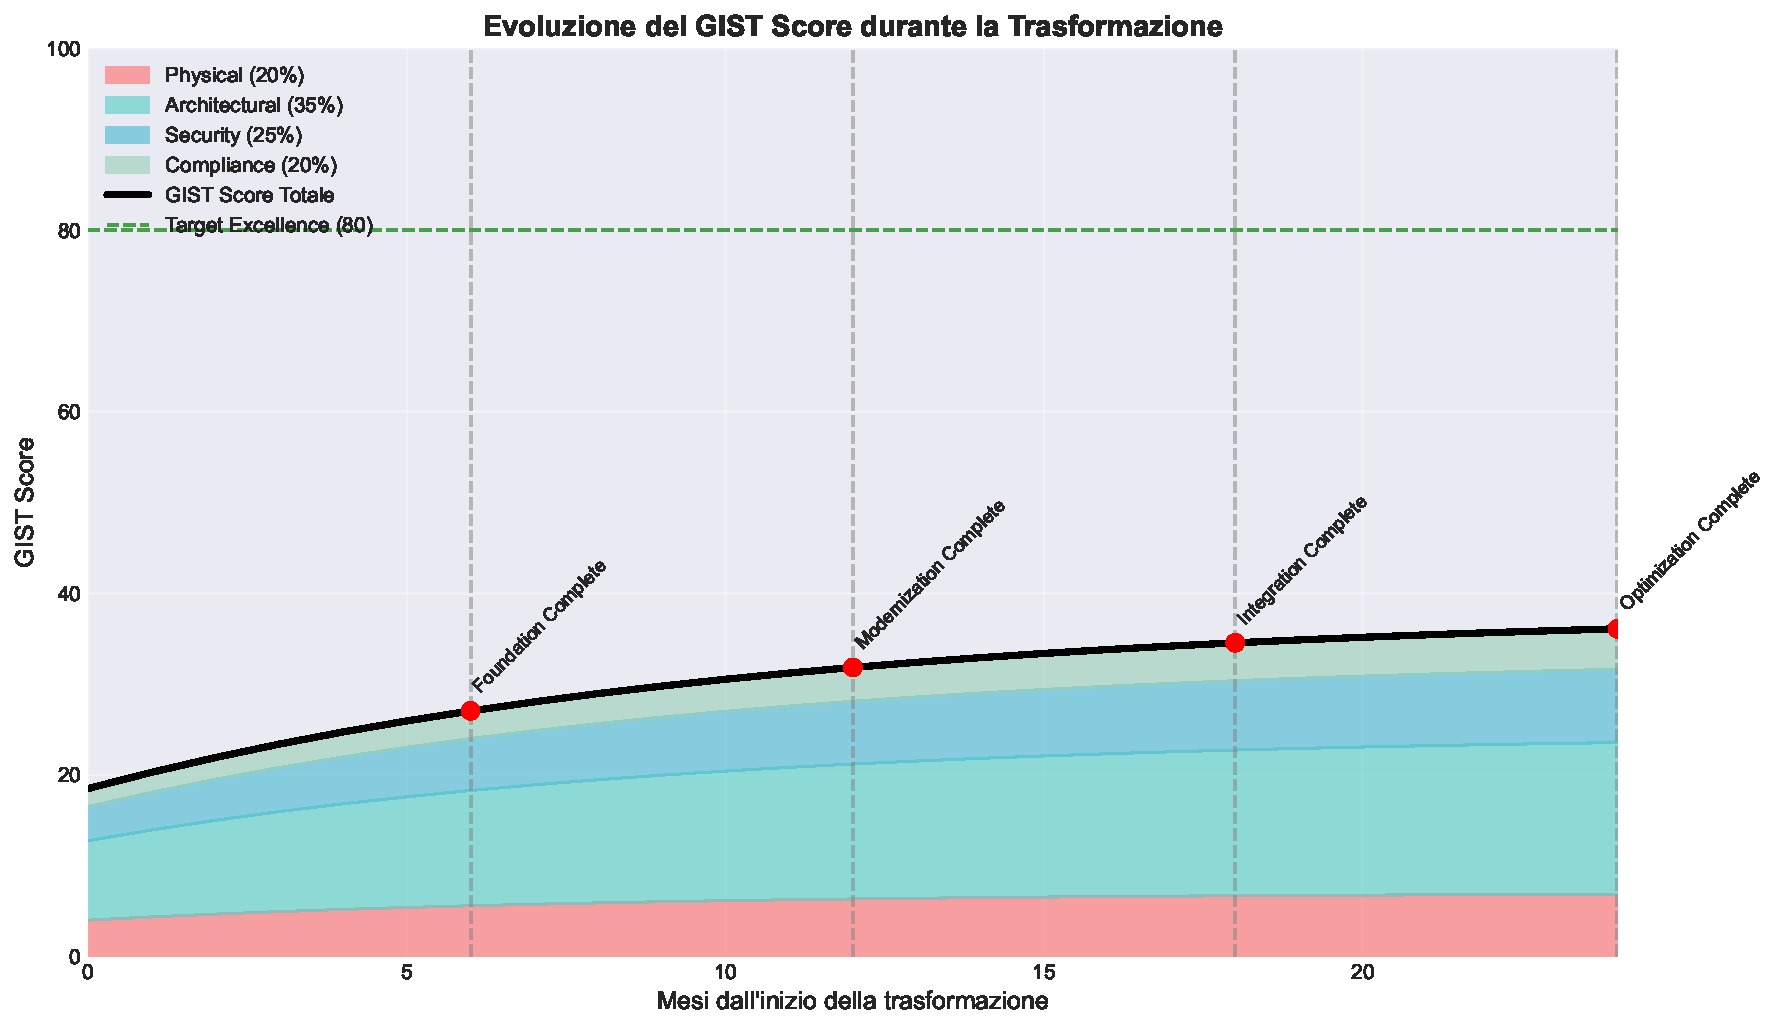
\includegraphics[width=0.9\textwidth]{thesis_figures/cap5/fig_5_6_gist_evolution.pdf}
% [PLACEHOLDER: Inserire framework per ricerca futura con aree prioritarie]
\caption{Framework per Ricerca Futura nel Dominio GDO Digital Transformation}
\label{fig:ricerca_futura}
\end{figure}

Le direzioni per ricerca futura includono l'estensione del framework GIST per incorporare esplicitamente dimensioni di sostenibilità ambientale, sempre più critiche nel contesto attuale. L'integrazione di metriche Environmental, Social, and Governance (ESG) nel framework di valutazione permetterebbe una visione più olistica del valore generato dalla trasformazione digitale.

L'applicazione di tecniche di Machine Learning per la predizione dinamica dei percorsi di trasformazione ottimali, basata su caratteristiche organizzative e contesto di mercato, potrebbe evolvere il framework da strumento di assessment statico a sistema di raccomandazione adattivo. Questo richiederebbe la costruzione di un dataset significativamente più ampio ma potrebbe rivoluzionare l'approccio alla pianificazione della trasformazione.

\subsection{Messaggio Finale per i Practitioner}

Per i leader IT e business nel settore della Grande Distribuzione Organizzata, il messaggio centrale di questa ricerca è chiaro: la trasformazione digitale sicura non è più differibile. Le evidenze presentate dimostrano che i benefici superano significativamente i costi quando la trasformazione è approcciata sistematicamente seguendo framework validati come GIST.

Il successo richiede però di superare l'approccio frammentato che caratterizza molte iniziative attuali. Investimenti isolati in tecnologie specifiche, per quanto avanzate, producono ritorni limitati se non inseriti in una trasformazione sistemica che consideri infrastruttura fisica, architettura IT, sicurezza e compliance come elementi interconnessi di un sistema unico.

La roadmap presentata fornisce un percorso validato che minimizza rischi e massimizza ritorni, ma la sua implementazione richiede commitment sostenuto del leadership, investimenti significativi ma giustificati, e soprattutto la volontà di affrontare il cambiamento culturale necessario. Le organizzazioni che agiranno decisivamente nei prossimi 12-18 mesi si posizioneranno come leader del retail digitale del prossimo decennio. Quelle che esiteranno rischiano di trovarsi in una spirale di obsolescenza da cui sarà sempre più difficile emergere.

La trasformazione digitale sicura non è un progetto IT, è una trasformazione del business che richiede l'IT come enabler fondamentale. Il framework GIST e le evidenze presentate in questa ricerca forniscono la base scientifica e pratica per intraprendere questo percorso con confidenza, basandosi su dati verificati e metodologie validate piuttosto che su intuizioni o mode tecnologiche. Il futuro del retail appartiene a chi saprà combinare l'efficienza digitale con la sicurezza sistemica e la conformità integrata. Il tempo per agire è ora.

%==========================================================================
% BIBLIOGRAFIA DEL CAPITOLO 5
%==========================================================================

% \bibliographystyle{IEEEtran}
% \bibliography{cap5_references}
% Note: Il file cap5_references.bib dovrebbe contenere le seguenti voci bibliografiche